\section{Data Transfer}

\begin{concept}{Data Transfer Overview}\\
ARM Cortex-M uses a load/store architecture:
\begin{itemize}
  \item Memory can only be accessed through load and store instructions
  \item All other operations work on registers
  \item Various addressing modes for flexible memory access
\end{itemize}
\end{concept}

\begin{formula}{Load Instructions}\\
Main load instructions for moving data into registers:
\begin{itemize}
  \item \textbf{MOVS} (Move and Set flags):
    \begin{itemize}
      \item Register to Register: \texttt{MOVS R1, R2}
      \item 8-bit immediate: \texttt{MOVS R1, \#0x1C}
      \item Constant: \texttt{MOVS R1, \#MyConst}
    \end{itemize}
  \item \textbf{LDR} (Load Register):
    \begin{itemize}
      \item 32-bit literal: \texttt{LDR R1, \#0xA1B2C3D4}
      \item PC-relative: \texttt{LDR R1, [PC, \#12]}
      \item Pseudo instruction: \texttt{LDR R1, =MyConst}
      \item Register indirect: \texttt{LDR R1, [R2]}
    \end{itemize}
  \item \textbf{LDRB} (Load Register Byte):
    \begin{itemize}
      \item Loads 8-bit value
      \item Bits 31 to 8 are set to zero
    \end{itemize}
  \item \textbf{LDRH} (Load Register Half-word):
    \begin{itemize}
      \item Loads 16-bit value
      \item Bits 31 to 16 are set to zero
    \end{itemize}
\end{itemize}
\end{formula}

\begin{formula}{Store Instructions}\\
Instructions for storing data from registers to memory:
\begin{itemize}
  \item \textbf{STR} (Store Register):
    \begin{itemize}
      \item Basic store: \texttt{STR R1, [R2]}
      \item With offset: \texttt{STR R1, [R2, \#0x04]}
    \end{itemize}
  \item \textbf{STRB} (Store Register Byte):
    \begin{itemize}
      \item Stores lowest 8 bits of register
    \end{itemize}
  \item \textbf{STRH} (Store Register Half-word):
    \begin{itemize}
      \item Stores lowest 16 bits of register
    \end{itemize}
\end{itemize}
\end{formula}

\begin{example2}{Memory Access Example}\\
Loading and storing array elements:

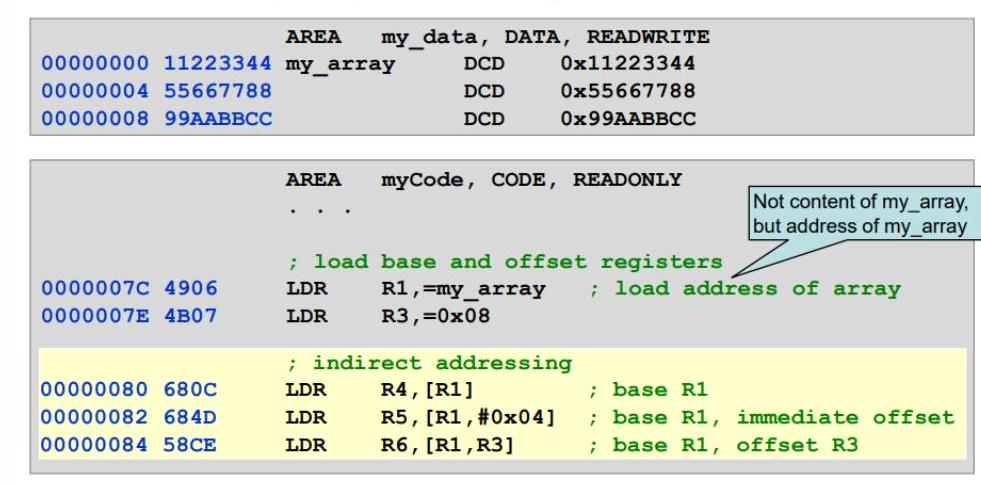
\includegraphics[width=\linewidth]{images/2024_12_29_79e6b22f503fb7b4f718g-03(1)}
\end{example2}

\begin{example2}{Memory Layout Example}\\
Memory layout for array elements and instructions:

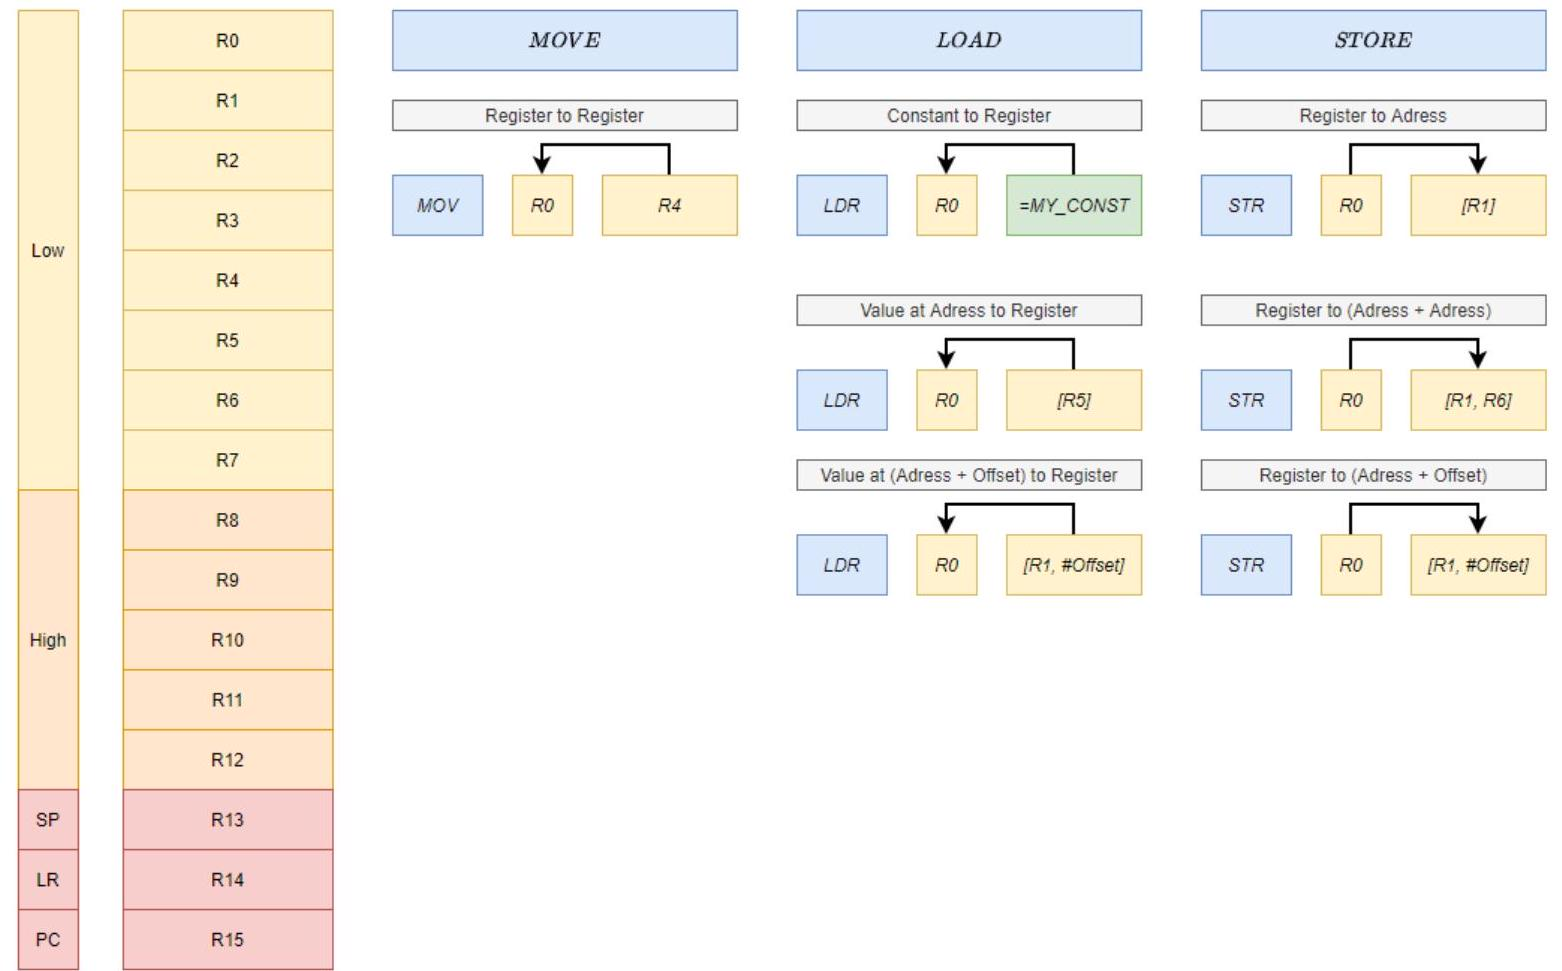
\includegraphics[width=\linewidth]{images/2024_12_29_79e6b22f503fb7b4f718g-03}
\end{example2}
\begin{remark}
Size considerations:
\begin{itemize}
  \item Array elements: 3 * 4 Bytes
  \item Instructions: 5 * 2 Bytes
  \item Literals (0x08): 1 * 4 Bytes
\end{itemize}
\end{remark}

\begin{KR}{Memory Access Patterns}\\
Steps for accessing memory:
\begin{enumerate}
  \item Determine required data size (byte, half-word, word)
  \item Choose appropriate load/store instruction
  \item Calculate correct memory address
  \item Consider alignment requirements
  \item Load/store data using proper addressing mode
\end{enumerate}
\end{KR}

\begin{example2}{Basic Data Transfer Operations}
Common data transfer operations:
\begin{lstlisting}[language=armasm, style=basesmol]
;Load operations
MOVS R1, #42      ;Load immediate value
MOVS R2, R1       ;Copy register
LDR  R3, =0x1234  ;Load 32-bit constant
LDR  R4, [R3]     ;Load from memory
LDRB R5, [R3, #1] ;Load byte with offset

;Store operations
STR  R1, [R2]     ;Store word
STRB R1, [R2, #4] ;Store byte with offset
STRH R1, [R2, R3] ;Store half-word with register offset
\end{lstlisting}
\end{example2}